\documentclass[12pt,a4paper]{article}
\usepackage[utf8]{inputenc}
\usepackage[T1]{fontenc}
\usepackage{graphicx}
\usepackage{geometry}
\usepackage{fancybox}
\usepackage{mdframed}
\usepackage{fancyhdr}
\usepackage{titlesec}
\usepackage{listings}
\usepackage{xcolor}
\usepackage[hidelinks]{hyperref}
\usepackage{booktabs}
\usepackage{array}
\usepackage{longtable}
\usepackage{enumitem}
\usepackage{setspace}
\usepackage{parskip}

% Page geometry with border
\geometry{margin=2.5cm}

% Page border
\usepackage{background}
\backgroundsetup{
    scale=1,
    color=black,
    opacity=1,
    angle=0,
    contents={%
        
\begin{tikzpicture}[remember picture, overlay]
            \draw[line width=1.5pt] 
                ([shift={(1cm,1cm)}]current page.south west) 
                rectangle 
                ([shift={(-1cm,-1cm)}]current page.north east);
        \end{tikzpicture}
    }
}
\usepackage{tikz}

% Set line spacing
\setstretch{1.3}

% Paragraph spacing
\setlength{\parskip}{0.8em}
\setlength{\parindent}{0pt}

% Header and footer
\pagestyle{fancy}
\fancyhf{}
\rhead{MarketPulse}
\cfoot{Jerome Wilson | Page \thepage}
\renewcommand{\headrulewidth}{0.4pt}
\renewcommand{\footrulewidth}{0.4pt}

% Code listing style
\lstset{
    basicstyle=\ttfamily\small,
    backgroundcolor=\color{gray!10},
    frame=single,
    breaklines=true,
    showstringspaces=false,
    tabsize=4
}

% Section formatting
\titleformat{\section}{\Large\bfseries}{\thesection.}{1em}{}
\titleformat{\subsection}{\large\bfseries}{\thesubsection}{1em}{}
\titlespacing*{\section}{0pt}{2em}{1em}
\titlespacing*{\subsection}{0pt}{1.5em}{0.8em}
\titlespacing*{\subsubsection}{0pt}{1em}{0.5em}

\begin{document}

% ==================== COVER PAGE ====================
\begin{titlepage}
    \centering
    \vspace*{3cm}
    
    {\Huge\bfseries MARKETPULSE\par}
    \vspace{1cm}
    {\Large AI-Powered Real-Time Stock Monitoring \& Insight Engine\par}
    \vspace{2cm}
    {\large SYSTEMS PROGRAMMING PROJECT REPORT\par}
    \vspace{4cm}
    {\large\bfseries Done By,\par}
    \vspace{0.5cm}
    {\Large Jerome Wilson\par}
    \vspace{0.3cm}
    {\large 2025SL70021\par}
    \vspace{2cm}
    {\large June 2026\par}
    
    \vfill
\end{titlepage}

% ==================== TABLE OF CONTENTS ====================
\tableofcontents
\newpage

% ==================== ABSTRACT ====================
\section{ABSTRACT}

\subsection{Abstract of the Project}

MarketPulse is an AI-powered real-time stock monitoring and insight engine developed as a comprehensive systems programming project. The application is designed for developers, students, and retail investors who require a lightweight, terminal-based tool to track stock markets without expensive graphical applications or browser-based platforms. Traditional stock monitoring tools present significant barriers including high costs (professional terminals like Bloomberg cost upwards of \$20,000 annually) and complex setup requirements.

MarketPulse addresses these challenges by providing a terminal-native application that fetches real-time stock prices from the Finnhub financial API, monitors multiple stocks simultaneously using parallel processing with \texttt{fork()} and \texttt{pipe()} system calls, detects price movements and triggers alerts using Unix signal handling mechanisms (SIGINT, SIGALRM, SIGCHLD), and generates intelligent AI-powered trading insights using the Groq API with the Llama 3.3 70B Versatile model. The parallel fetching architecture reduces data retrieval time by approximately 10x compared to sequential fetching.

The project combines network programming (\texttt{socket()}, \texttt{connect()}, SSL/TLS via OpenSSL), process management (\texttt{fork()}, \texttt{pipe()}, \texttt{waitpid()}), signal handling (\texttt{signal()}, \texttt{sigaction()}, \texttt{alarm()}), memory-mapped files (\texttt{mmap()}, \texttt{msync()}), terminal control (\texttt{tcgetattr()}, \texttt{tcsetattr()}), and I/O multiplexing (\texttt{select()}) into a single integrated platform. The application supports both US markets (S\&P 500 via NYSE/NASDAQ) and Indian markets (NIFTY50 via NSE/BSE) with automatic currency detection and timezone-aware market status display.

\newpage

% ==================== INTRODUCTION ====================
\section{INTRODUCTION}

\subsection{Introduction to the Project}

Stock market monitoring is essential for investors, traders, and financial analysts. However, existing tools present significant challenges for various user groups:

\subsubsection{For Developers and System Administrators:}
\begin{itemize}[itemsep=0.3em]
    \item Working primarily in terminals, switching to browser-based tools breaks workflow
    \item No way to monitor stocks while coding or deploying
    \item Existing CLI tools require manual JSON parsing
\end{itemize}

\subsubsection{For Retail Investors:}
\begin{itemize}[itemsep=0.3em]
    \item Professional tools like Bloomberg Terminal cost \$20,000+/year
    \item Free tools are cluttered with ads and unnecessary features
    \item No real-time alerts for price movements
\end{itemize}

\subsubsection{For Students:}
\begin{itemize}[itemsep=0.3em]
    \item Learning system programming concepts through practical applications
    \item Understanding process management, IPC, and network programming
    \item Gaining exposure to AI integration in systems software
\end{itemize}

MarketPulse was developed to eliminate these barriers by introducing a terminal-native stock monitoring solution with AI-assisted insights and real-time alerts.

\newpage

% ==================== PROBLEM STATEMENT ====================
\section{PROBLEM STATEMENT}

\subsection{Problem Statement of the Project}

Traditional stock monitoring solutions are not designed with developers and terminal users as a primary concern.

\subsubsection{Major Limitations Include:}

\textbf{Accessibility Challenges}
\begin{itemize}[itemsep=0.3em]
    \item Heavy dependence on graphical interfaces
    \item Expensive subscription requirements
    \item Complex setup and configuration
    \item No terminal-based solutions
\end{itemize}

\textbf{Technical Challenges}
\begin{itemize}[itemsep=0.3em]
    \item Sequential data fetching is slow for multiple stocks
    \item API rate limiting from financial data providers
    \item Complex SSL/TLS handshaking for secure connections
    \item No persistent price history across sessions
\end{itemize}

\textbf{User Experience Challenges}
\begin{itemize}[itemsep=0.3em]
    \item Raw JSON output is hard to read
    \item No visual indicators for trends
    \item No keyboard controls for interaction
    \item Blocking I/O prevents responsive UI
\end{itemize}

MarketPulse aims to solve these issues by enabling users to monitor stocks directly from the terminal with parallel fetching, AI insights, and real-time alerts.

\newpage

% ==================== PROJECT OBJECTIVES ====================
\section{PROJECT OBJECTIVES}

\subsection{Objectives of the Project}

\subsubsection{Primary Objective}
To develop an AI-assisted stock monitoring system that demonstrates core system programming concepts while providing real trading value to developers, students, and retail investors.

\subsubsection{Secondary Objectives}
\begin{itemize}[itemsep=0.3em]
    \item Provide real-time stock price fetching from external APIs
    \item Enable multi-stock monitoring with parallel processing
    \item Offer AI-powered technical analysis and trading insights
    \item Implement price alert system with signal handling
    \item Support both US (S\&P 500) and Indian (NIFTY50) markets
    \item Maintain persistent price history using memory-mapped files
    \item Create intuitive terminal UI with keyboard controls
\end{itemize}

\newpage

% ==================== SYSTEM ARCHITECTURE ====================
\section{SYSTEM ARCHITECTURE}

\subsection{Architecture}

\begin{figure}[h]
    \centering
    % Try one of these paths depending on where your image is located:
    % Option 1: If image is in 'images' folder
    % \includegraphics[width=0.7\textwidth]{images/arch-image.jpeg}
    % Option 2: If image is in root folder (same level as .tex file)
    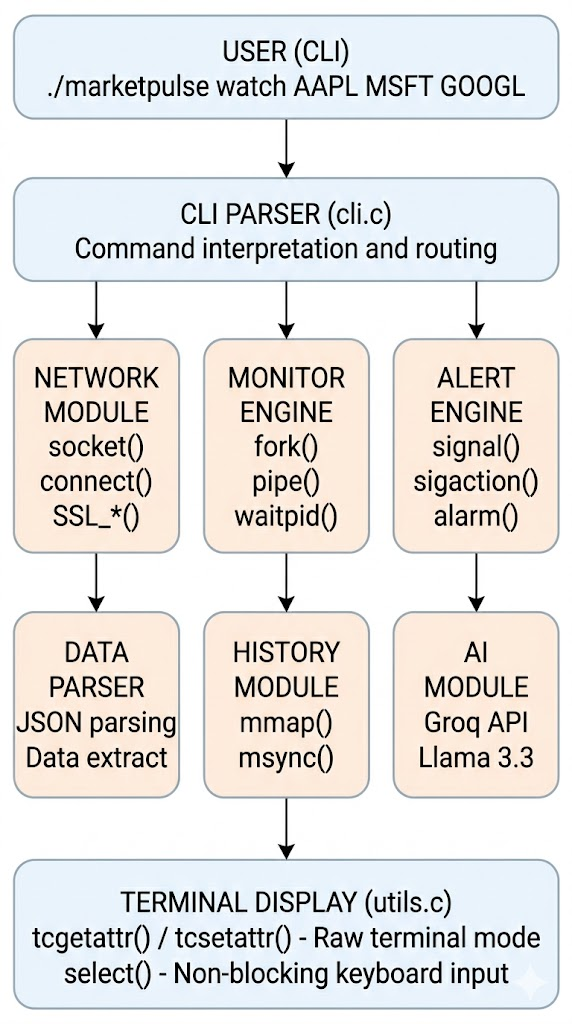
\includegraphics[width=0.7\textwidth]{arch-img.jpeg}
    % Option 3: If using .jpg extension
    % \includegraphics[width=0.7\textwidth]{arch-image.jpg}
    \caption{MarketPulse System Architecture}
\end{figure}

\subsection{Layer Description}

\textbf{Input Layer:} User CLI commands and keyboard input during monitoring

\textbf{Processing Layer:} CLI parsing, network communication, parallel stock fetching with fork/pipe, signal-based alert monitoring

\textbf{Data Layer:} JSON parsing for API responses, memory-mapped price history, AI insight generation

\textbf{Output Layer:} Terminal UI with colors and charts, sparkline price visualization

\newpage

% ==================== TECHNOLOGIES USED ====================
\section{TECHNOLOGIES USED}

\subsection{Technologies Used}

\begin{longtable}{|p{5cm}|p{8cm}|}
\hline
\textbf{Technology} & \textbf{Purpose} \\
\hline
\endfirsthead
\hline
\textbf{Technology} & \textbf{Purpose} \\
\hline
\endhead
C Programming & Core implementation \\
\hline
Linux/macOS System Calls & Process and file management \\
\hline
OpenSSL & HTTPS/TLS encryption \\
\hline
Finnhub API & Real-time stock data \\
\hline
Groq API & AI-powered insights \\
\hline
Llama 3.3 Model & Natural language analysis \\
\hline
fork() & Process creation for parallel fetching \\
\hline
pipe() & Inter-process communication \\
\hline
waitpid() & Process synchronization \\
\hline
socket() & Network socket creation \\
\hline
connect() & TCP connection establishment \\
\hline
signal() / sigaction() & Signal handling \\
\hline
alarm() & Timer-based alerts \\
\hline
mmap() / msync() & Memory-mapped file persistence \\
\hline
select() & I/O multiplexing \\
\hline
tcgetattr() / tcsetattr() & Terminal raw mode \\
\hline
\end{longtable}

MarketPulse extensively utilizes Linux process management concepts including fork-exec architecture, IPC mechanisms, and signal handling.

\newpage

% ==================== AI COMPONENTS ====================
\section{AI COMPONENTS}

\subsection{AI Integration Overview}

MarketPulse integrates artificial intelligence through the Groq API, utilizing the Llama 3.3 70B Versatile model for intelligent stock analysis and trading insights.

\subsection{Single Stock AI Analysis}

When fetching a single stock, MarketPulse automatically generates AI-powered insights.

\textbf{Example:}
\begin{lstlisting}
Command: ./marketpulse AAPL

AI Commentary:
AAPL shows bullish momentum with price above key moving averages.
Support at $185, resistance at $195. Consider holding or adding
on dips below $187.
\end{lstlisting}

\textbf{Features:}
\begin{itemize}[itemsep=0.3em]
    \item Trend assessment (Bullish/Bearish/Neutral)
    \item Support and resistance levels
    \item Trading suggestions
    \item Automatic with every fetch - no extra command needed
\end{itemize}

\subsection{Market Overview AI}

Press 'I' in watch mode to get AI-powered market analysis.

\textbf{Features:}
\begin{itemize}[itemsep=0.3em]
    \item Overall market sentiment
    \item Top performers analysis
    \item Actionable trading advice
    \item Market-wide insights across all watched stocks
\end{itemize}

\subsection{Technical Analysis}

MarketPulse performs technical analysis including:
\begin{itemize}[itemsep=0.3em]
    \item Moving Averages (MA5, MA10)
    \item RSI (Relative Strength Index)
    \item Volatility percentage
    \item Golden Cross / Death Cross signal detection
\end{itemize}

\subsection{Deep Analysis Mode}

\begin{lstlisting}
Command: ./marketpulse insight NVDA
\end{lstlisting}

Provides comprehensive technical analysis with detailed AI commentary and signal detection.

\newpage

% ==================== FEATURES AND FUNCTIONALITIES ====================
\section{FEATURES AND FUNCTIONALITIES}

\subsection{Single Stock Fetch}

\begin{lstlisting}
./marketpulse AAPL
\end{lstlisting}

\textbf{Features:}
\begin{itemize}[itemsep=0.3em]
    \item Real-time price from Finnhub API
    \item Price change (absolute and percentage)
    \item Open, High, Low, Previous Close
    \item Automatic AI-powered insights
    \item Market status (OPEN/CLOSED)
\end{itemize}

\subsection{Multi-Stock Watch Mode}

\begin{lstlisting}
./marketpulse watch AAPL MSFT GOOGL
\end{lstlisting}

\textbf{Features:}
\begin{itemize}[itemsep=0.3em]
    \item Parallel fetching using fork() and pipe()
    \item Real-time updates every 5 seconds
    \item Sparkline charts showing price history
    \item Color-coded trend indicators (green/red)
    \item Keyboard controls (Q, S, P, +, -)
\end{itemize}

\subsection{Index Monitoring}

\begin{lstlisting}
./marketpulse watch sp500    # US S&P 500 stocks
./marketpulse watch nifty50  # Indian NIFTY50 stocks
\end{lstlisting}

\textbf{Features:}
\begin{itemize}[itemsep=0.3em]
    \item Predefined stock groups
    \item Automatic currency detection (\$ or Rs.)
    \item Timezone-aware market status
    \item Regional market hours detection
\end{itemize}

\subsection{Price Alert System}

\begin{lstlisting}
./marketpulse alert AAPL 190
\end{lstlisting}

\textbf{Features:}
\begin{itemize}[itemsep=0.3em]
    \item Signal-based threshold monitoring
    \item Visual terminal flash alerts
    \item Audio bell notifications
    \item Bidirectional threshold crossing detection
    \item Graceful shutdown with Ctrl+C
\end{itemize}

\subsection{Keyboard Controls}

\begin{tabular}{|c|l|}
\hline
\textbf{Key} & \textbf{Action} \\
\hline
Q & Quit monitoring \\
\hline
S & Sort by change percentage \\
\hline
I & Show AI market insights \\
\hline
P & Pause/Resume updates \\
\hline
+ & Faster refresh rate \\
\hline
- & Slower refresh rate \\
\hline
Esc & Close insights panel \\
\hline
\end{tabular}

\subsection{Visual Features}
\begin{itemize}[itemsep=0.3em]
    \item Color-coded price changes (green for up, red for down)
    \item Sparkline charts using Unicode block elements
    \item Trend arrows
    \item Market status indicators
\end{itemize}

\newpage

% ==================== CORE CONCEPTS ====================
\section{CORE CONCEPTS}

\subsection{Core Linux Concepts Implemented}

\subsubsection{Process Management}
\begin{itemize}[itemsep=0.3em]
    \item \texttt{fork()} - Create child processes for parallel stock fetching
    \item \texttt{waitpid()} - Synchronize parent-child processes, prevent zombies
    \item \texttt{exit()} - Terminate child processes
\end{itemize}

\subsubsection{Inter-Process Communication}
\begin{itemize}[itemsep=0.3em]
    \item \texttt{pipe()} - Unidirectional data channel between processes
    \item \texttt{mkfifo()} - Named pipes for external tool integration
\end{itemize}

\subsubsection{Network Programming}
\begin{itemize}[itemsep=0.3em]
    \item \texttt{socket()} - Create network communication endpoint
    \item \texttt{connect()} - Establish TCP connection to API servers
    \item \texttt{getaddrinfo()} - DNS resolution
\end{itemize}

\subsubsection{Signal Handling}
\begin{itemize}[itemsep=0.3em]
    \item \texttt{signal()} - Basic signal handling (SIGPIPE)
    \item \texttt{sigaction()} - Advanced signal handling (SIGINT, SIGALRM, SIGCHLD)
    \item \texttt{alarm()} - Timer-based periodic price checking
    \item \texttt{kill()} - Send signals to background processes
\end{itemize}

\subsubsection{Memory Management}
\begin{itemize}[itemsep=0.3em]
    \item \texttt{mmap()} - Memory-mapped files for persistent price history
    \item \texttt{msync()} - Synchronize memory to disk
\end{itemize}

\subsubsection{Terminal Control}
\begin{itemize}[itemsep=0.3em]
    \item \texttt{tcgetattr()} - Get terminal attributes
    \item \texttt{tcsetattr()} - Set terminal to raw mode for immediate key response
\end{itemize}

\subsubsection{I/O Multiplexing}
\begin{itemize}[itemsep=0.3em]
    \item \texttt{select()} - Non-blocking keyboard input checking
\end{itemize}

\newpage

% ==================== PROJECT WORKFLOW ====================
\section{PROJECT WORKFLOW}

\subsection{Project Workflow}

\textbf{Step 1:} User enters command (e.g., \texttt{./marketpulse watch AAPL MSFT})

\textbf{Step 2:} CLI parser interprets command and extracts symbols

\textbf{Step 3:} Terminal switched to raw mode using \texttt{tcsetattr()}

\textbf{Step 4:} For each stock: \texttt{socket()} creates TCP endpoint, \texttt{connect()} establishes connection, \texttt{SSL\_connect()} performs TLS handshake

\textbf{Step 5:} \texttt{fork()} creates child process for each stock, each child fetches independently via HTTPS, \texttt{pipe()} transfers data back to parent, \texttt{waitpid()} synchronizes all children

\textbf{Step 6:} JSON response parsed to extract price data, price added to mmap'd history file, \texttt{msync()} persists to disk

\textbf{Step 7:} Stock data sent to Groq API, Llama 3.3 generates trading insights, response parsed and formatted

\textbf{Step 8:} Clear screen with ANSI codes, render table with colors, draw sparkline charts, show trend indicators

\textbf{Step 9:} \texttt{select()} checks for input without blocking, handle Q/S/P/+/- keys, loop back to Step 5 after refresh interval

\textbf{Step 10:} Restore terminal settings, close mmap'd files, exit gracefully

\newpage

% ==================== CHALLENGES ====================
\section{CHALLENGES}

\subsection{Challenges Faced During Development}

\subsubsection{Challenge 1: High Latency in Sequential Fetching}

\textbf{Problem:} Fetching 10 stocks sequentially took 10-15 seconds due to DNS resolution, TCP 3-way handshake, SSL/TLS handshake, and HTTP request/response.

\textbf{Solution:} Implemented parallel fetching using \texttt{fork()} and \texttt{pipe()}:

\begin{lstlisting}[language=C]
for (int i = 0; i < stock_count; i++) {
    pipe(pipes[i]);
    pids[i] = fork();
    if (pids[i] == 0) {
        // Child fetches one stock
        fetch_stock_quote(symbols[i], &stock);
        write(pipes[i][1], &stock, sizeof(stock));
        exit(0);
    }
}
\end{lstlisting}

\textbf{Result:} 10 stocks now fetch in ~1-2 seconds.

\subsubsection{Challenge 2: API Rate Limiting}

\textbf{Problem:} Finnhub API limits requests to 60 calls/minute. With 10 stocks refreshing every 5 seconds, we exceeded the limit.

\textbf{Solution:}
\begin{itemize}[itemsep=0.3em]
    \item Staggered requests with \texttt{usleep()} between fetches
    \item Implemented token bucket rate limiter
    \item Added simulated data fallback when quota exhausted
    \item Caching of recent responses
\end{itemize}

\subsubsection{Challenge 3: SSL/TLS Complexity}

\textbf{Problem:} Financial APIs require HTTPS. In C, this requires OpenSSL library initialization, SSL context creation, certificate verification, and proper error handling (SSL errors don't set errno).

\textbf{Solution:} Created robust SSL wrapper functions with proper initialization, error handling, and cleanup to prevent memory leaks.

\subsubsection{Challenge 4: JSON Parsing Without Libraries}

\textbf{Problem:} C has no built-in JSON parser. External libraries add dependencies.

\textbf{Solution:} Built custom lightweight JSON parser using string matching:

\begin{lstlisting}[language=C]
double extract_json_double(const char *json, const char *key) {
    char search[64];
    snprintf(search, sizeof(search), "\"%s\":", key);
    char *pos = strstr(json, search);
    if (pos) {
        pos += strlen(search);
        return atof(pos);
    }
    return 0.0;
}
\end{lstlisting}

\subsubsection{Challenge 5: Terminal Raw Mode and Keyboard Input}

\textbf{Problem:} Default terminal mode is line-buffered - user must press Enter for input. This prevents responsive keyboard controls.

\textbf{Solution:} Used \texttt{tcsetattr()} to switch to raw mode and \texttt{select()} for non-blocking input:

\begin{lstlisting}[language=C]
raw.c_lflag &= ~(ICANON | ECHO);
tcsetattr(STDIN_FILENO, TCSANOW, &raw);
\end{lstlisting}

\newpage

% ==================== PROJECT AND AI ====================
\section{PROJECT AND AI}

\subsection{Project Journey and AI Usage}

A significant part of MarketPulse's development involved iterative design, debugging, optimization, and feature enhancement using AI-assisted development workflows.

\subsection{AI Tools Used}

\subsubsection{Cline (AI Development Assistant)}
Used throughout the development process for:
\begin{itemize}[itemsep=0.3em]
    \item Architecture planning and module design
    \item Code generation and implementation
    \item Debugging complex issues
    \item Documentation generation
\end{itemize}

\subsubsection{Groq API (Runtime AI)}
Integrated into the application for:
\begin{itemize}[itemsep=0.3em]
    \item Real-time stock analysis
    \item Trading insight generation
    \item Market sentiment analysis
\end{itemize}

\subsection{AI Assistance Used For}

\textbf{System Design}
\begin{itemize}[itemsep=0.3em]
    \item Architecture planning
    \item Module decomposition
    \item System call selection
    \item Data flow design
\end{itemize}

\textbf{Feature Development}
\begin{itemize}[itemsep=0.3em]
    \item Network module implementation
    \item Parallel fetching with fork/pipe
    \item Signal-based alert system
    \item Memory-mapped history
    \item Terminal UI rendering
\end{itemize}

\textbf{Debugging}
\begin{itemize}[itemsep=0.3em]
    \item Fork-related issues
    \item SSL/TLS handshaking problems
    \item JSON parsing edge cases
    \item Race conditions in IPC
    \item Terminal mode restoration
\end{itemize}

\textbf{Documentation and Presentation}
\begin{itemize}[itemsep=0.3em]
    \item Technical explanations
    \item Project documentation
    \item Presentation content
    \item Architecture diagrams
\end{itemize}

The final implementation, integration, testing, debugging, and feature customization were performed by the developer. AI assistance was used as a tool to accelerate development and improve code quality, but all design decisions, testing, and final implementation were done by the developer.

\newpage

% ==================== FUTURE ENHANCEMENTS ====================
\section{FUTURE ENHANCEMENTS}

\subsection{Future Enhancements}

Planned features include:

\subsubsection{WebSocket Support}
\begin{itemize}[itemsep=0.3em]
    \item True real-time streaming instead of polling
    \item Lower latency price updates
    \item Reduced API calls
\end{itemize}

\subsubsection{Portfolio Tracking}
\begin{itemize}[itemsep=0.3em]
    \item Track owned stocks
    \item Calculate profit/loss
    \item Portfolio performance metrics
\end{itemize}

\subsubsection{Multiple AI Models}
\begin{itemize}[itemsep=0.3em]
    \item GPT-4 integration
    \item Claude integration
    \item Model comparison
\end{itemize}

\subsubsection{Mobile Notifications}
\begin{itemize}[itemsep=0.3em]
    \item Push notifications via services
    \item SMS alerts for critical prices
    \item Email notifications
\end{itemize}

\subsubsection{Cryptocurrency Support}
\begin{itemize}[itemsep=0.3em]
    \item Bitcoin, Ethereum monitoring
    \item Crypto exchange integration
    \item 24/7 market support
\end{itemize}

\newpage

% ==================== APPLICATIONS ====================
\section{APPLICATIONS}

\subsection{Real-World Applications}

MarketPulse can be used as:

\subsubsection{Retail Investors}
Quick terminal-based market monitoring without expensive subscriptions.

\subsubsection{Day Traders}
Real-time alerts and AI insights for trading decisions.

\subsubsection{Developers}
Monitor stocks while coding without leaving the terminal.

\subsubsection{Students}
Learning system programming concepts through practical application.

\subsubsection{Quant Analysts}
Building automated trading systems and analysis tools.

\subsubsection{Financial Educators}
Teaching market concepts with live data.

\newpage

% ==================== CONCLUSION ====================
\section{CONCLUSION}

\subsection{Conclusion}

MarketPulse successfully demonstrates how system programming concepts can be combined with modern AI to create a powerful, practical application.

\subsubsection{Key Achievements:}
\begin{itemize}[itemsep=0.3em]
    \item Implemented 15+ system calls (fork, pipe, socket, signal, mmap, select, etc.)
    \item Parallel processing with fork/pipe architecture reduces fetch time by 10x
    \item Signal-based alert system with graceful shutdown
    \item AI integration using Groq API with Llama 3.3 for intelligent trading insights
    \item Dual market support (US and India) with automatic currency/timezone detection
    \item Intuitive terminal-based UI with keyboard controls and sparkline charts
    \item Persistent price history using memory-mapped files
\end{itemize}

\begin{center}
\textbf{Project Repository:}\\
\url{https://github.com/jerome-wilson/marketpulse}
\end{center}

\end{document}